

DigitalOcean jest znanym dostawcą chmury obliczeniowej który oferuje infrastrukturę zgodną z zasadą IaaS (ang. Infrastructure as a Service) dla twórców oprogramowania. Jest bardzo popularny i znakomicie konkuruje z AWS (ang. Amazon Web Services) czy też Google Compute Engine.

W celu uruchomienia środowiska programiści uruchamiają instancję prywatnej maszyny wirtualnej (VM) która w DigitalOcean nosi nazwę droplet(kropelka). Użytkownik może wybrać wielkość kropelki, region geograficzny i centrum danych w którym będziue ona działać oraz system operacyjny z rodziny Linux.
Można jednocześnie użyć swoich obrazów do postawienia gotowego środowiska uruchomieniowego.

Aktualnie dostawca oferuje czternaście rozmiarów kropli. Najmniejszy rozmiar zaczyna się od 1GB pamięci RAM z 1 procesorem i 25GB pamięci SSD, taki układ to koszt 5\$ miesięcznie ( rys. \ref{fig:digitalocean}). Wraz ze wzrostem specyfikacji rośnie również cena, aby maksymalnie osiągnąć 960\$ za 192GB pamięci RAM z 32 procesorami i 12TB pamięci SSD.

Deweloperzy używają systemu DigitalOcean do zarządzania i monitorowania kropli za pomocą panelu sterowania i API open source. Panel kontrolny umożliwia deweloperom skalowanie i przebudowę kropli na podstawie zmian w obciążeniu pracą oraz wykonywanie kopii zapasowych i przekierowywanie ruchu sieciowego pomiędzy kropelkami.

DigitalOcean został założony w 2011 roku przez Bena Ureckiego, Moiseya Ureckiego, Mitcha Wainera, Jeffa Carra i Aleca Hartmana. Siedziba firmy znajduje się w Nowym Jorku.


\begin{figure}[H]
    \centering
    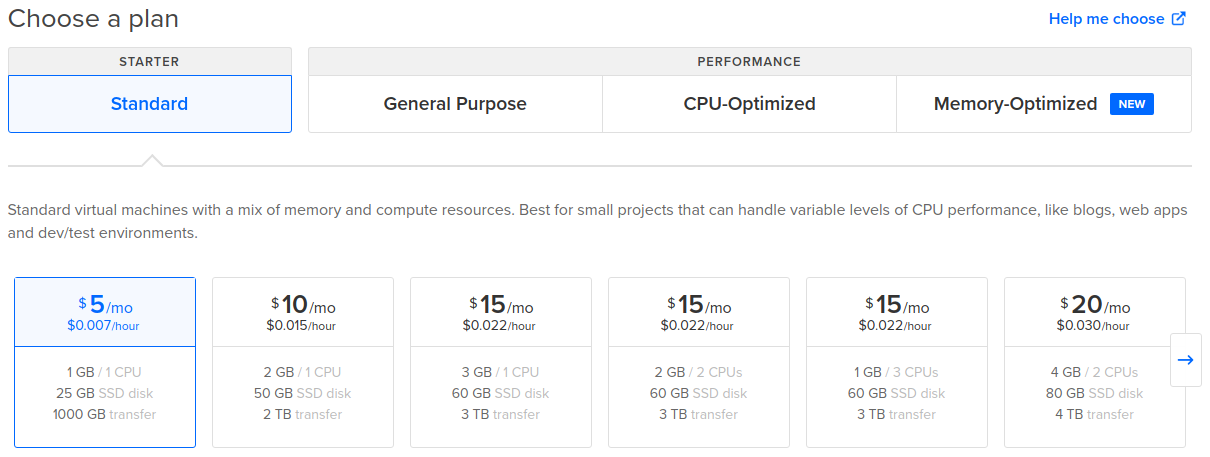
\includegraphics[width=6in]{images/digitalocean.png}
    \caption{Wybór mozliwych konfiguracji na stronie https://cloud.digitalocean.com \label{fig:digitalocean}}
\end{figure}